\hypertarget{setup}{%
\section{Setup}\label{setup}}

This project is a list of apps that they combine custom GUI for the PAT
system.

\textbf{Requirements}

\includegraphics{https://img.shields.io/static/v1?label=cpp\&message=11\&color=007bff}

\includegraphics{https://img.shields.io/static/v1?label=cmake\&message=3.16\&color=007bff}

\includegraphics{https://img.shields.io/static/v1?label=git\&message=2.0\&color=007bff}

\includegraphics{https://img.shields.io/static/v1?label=Doxygen\&message=1.8.13\&color=007bff}

\includegraphics{https://img.shields.io/static/v1?label=Sphinx\&message=3.0.2\&color=007bff}

\includegraphics{https://img.shields.io/static/v1?label=OS\&message=Win\&color=28a745\%22}

\hypertarget{generality}{%
\subsection{Generality}\label{generality}}

\hypertarget{import}{%
\subsubsection{Import}\label{import}}

Import as an external library into your project by copy-paste the
following lines in your \texttt{config.json}.

\begin{Shaded}
\begin{Highlighting}[]
\FunctionTok{\{}
  \DataTypeTok{"name"}     \FunctionTok{:} \StringTok{"PATSetup"}\FunctionTok{,}
  \DataTypeTok{"path"}     \FunctionTok{:} \StringTok{"gitlab.dei.unipd.it/PAT/Setup.git"}\FunctionTok{,}
  \DataTypeTok{"tag"}      \FunctionTok{:} \StringTok{"HEAD"}\FunctionTok{,}
  \DataTypeTok{"available"}\FunctionTok{:} \StringTok{"YES"}\FunctionTok{,}
  \DataTypeTok{"getGui"}   \FunctionTok{:} \StringTok{"YES"}
\FunctionTok{\}}
\end{Highlighting}
\end{Shaded}

\hypertarget{prerequisites}{%
\subsubsection{Prerequisites}\label{prerequisites}}

The following libraries are auto fetched from the gitlab.dei.unipd.it
host (ask the owner of this repo to become a member):

\begin{itemize}
\tightlist
\item
  \href{https://gitlab.dei.unipd.it/PAT/Controller.git}{Controller}
  1.0.0
\end{itemize}

These other libraries need to be installed manually in your system:

\begin{itemize}
\tightlist
\item
  \href{https://www.qt.io/}{Qt} 5.14.2
\end{itemize}

The library documentation is generated through
\href{http://www.doxygen.nl/download.html}{Doxygen 1.8.13}. Additional
documentation in the \texttt{index} folder is generated through the
\href{https://www.anaconda.com/products/individual}{python3} package
\href{https://www.sphinx-doc.org/en/master/}{Sphinx} using the following
extensions (which you can install through pip3):

\begin{itemize}
\tightlist
\item
  \href{https://pypi.org/project/Sphinx/}{Sphinx 3.0.2}
\item
  \href{https://sphinx-rtd-theme.readthedocs.io/en/stable/}{Sphinx read
  the doc theme} (to use the read the doc theme for html documentation)
\item
  \href{https://pypi.org/project/breathe/}{Breathe} (to use the xml
  output of doxygen)
\item
  \href{https://pypi.org/project/sphinx-markdown-builder/}{Sphinx-markdown-builder}
  (to generate the markdown version for gitlab wiki)
\end{itemize}

\texttt{pip3\ install\ Sphinx\ sphinx\_rtd\_theme\ breathe\ sphinx-markdown-builder}

\hypertarget{usage}{%
\subsection{Usage}\label{usage}}

In this repo you can create your own GUI for the PAT system in the
\texttt{apps} folder. As reference you can use one of the already
defined apps. There is no need to explain additional things because in
this repository you want to compose ready-made pieces and not create new
ones.

\hypertarget{uml}{%
\subsection{UML}\label{uml}}

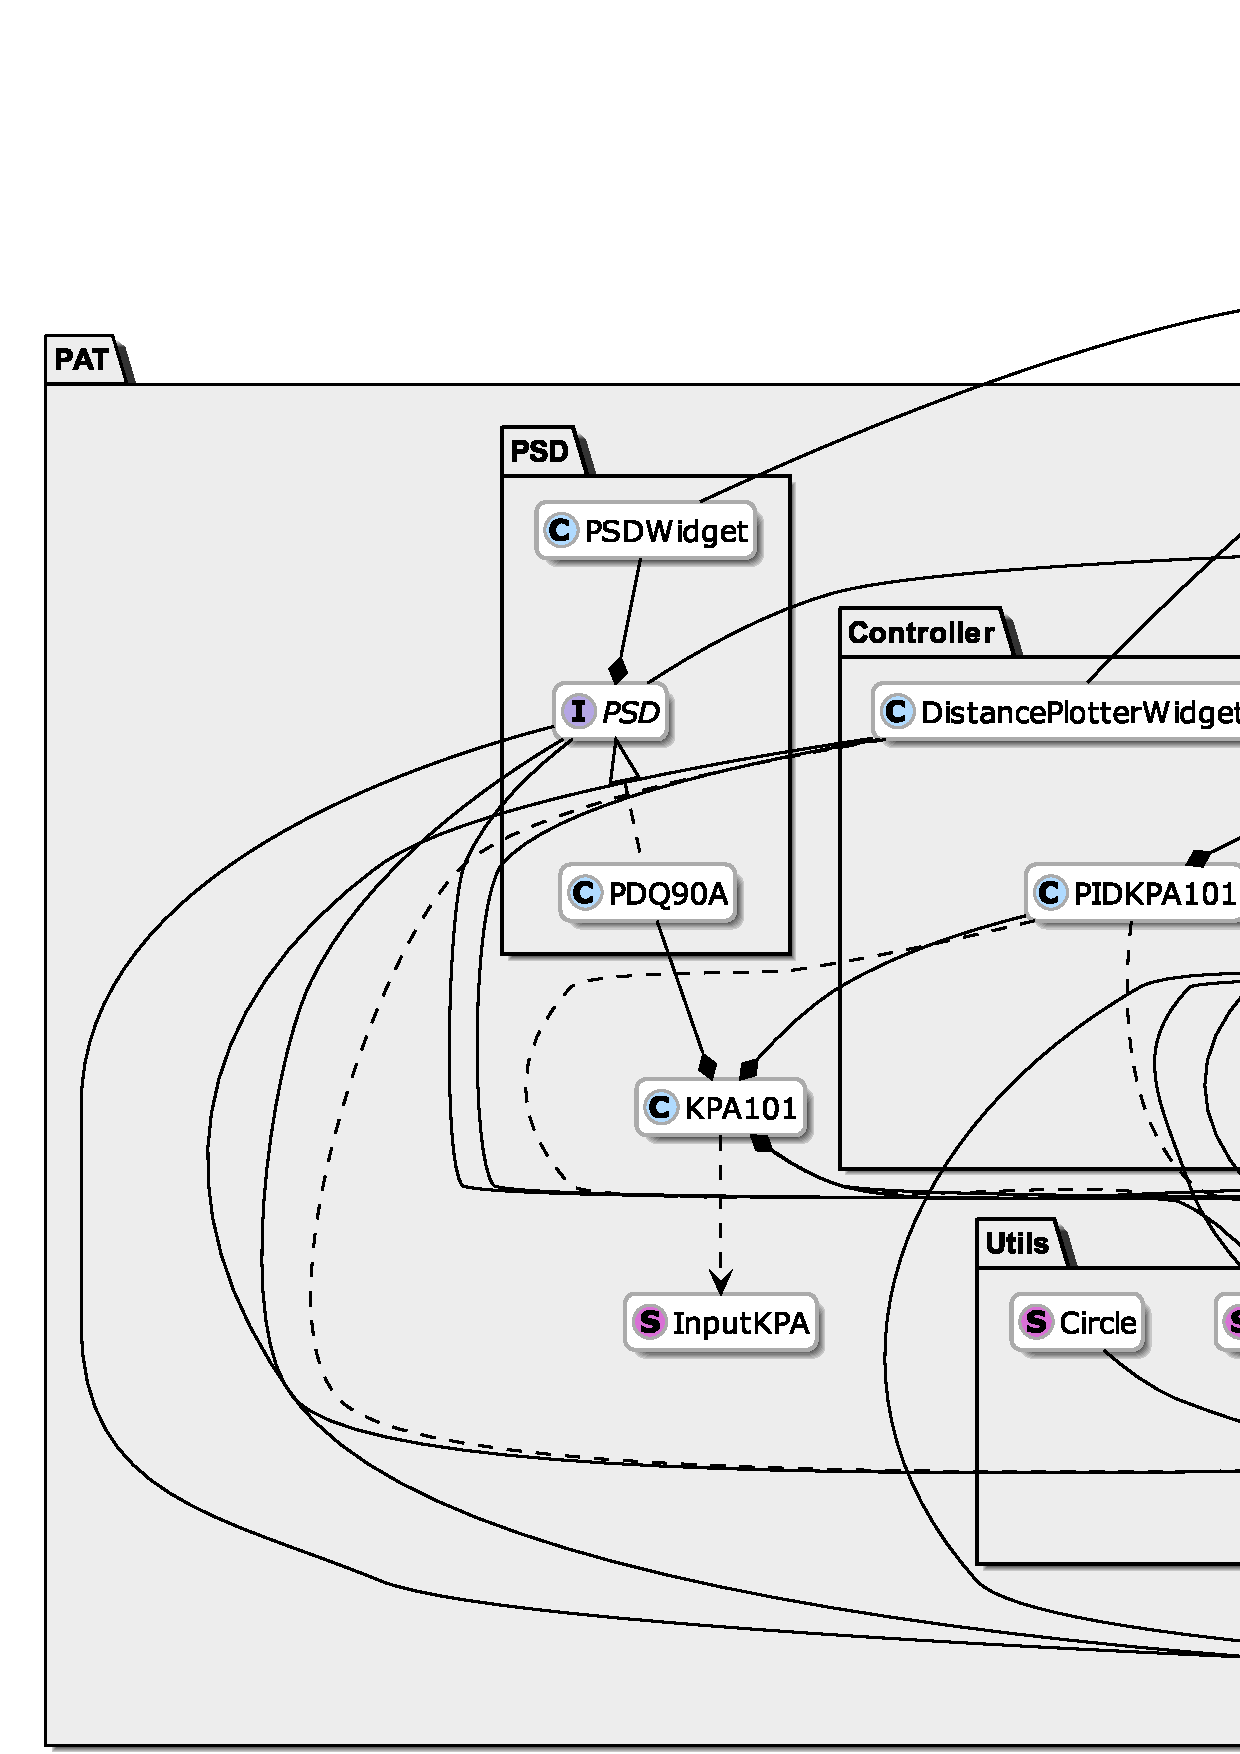
\includegraphics[width=8.33333in,height=\textheight]{https://gitlab.dei.unipd.it/pat/docs/-/raw/4da37d1e14c960824565fc73d9bca1143e667907/out/repositories/Setup/Setup.svg}
